\documentclass[letterpaper,10pt]{article}
\usepackage{biblatex} %Imports biblatex package
\addbibresource{references.bib} %Import the bibliography file
\usepackage{graphicx} % Required for inserting images
\usepackage{float}

\title{What strategies makes alpine ski racers perform well on flats in slalom and what is a good training strategy to learn these strategies}
\author{Christian Magelssen}
\date{January 2024}

\begin{document}

\maketitle

\section{Background}

Jeg har skrevet en del her, men har kommentert ut. Men planen er bare å gi en kort intro til prosjektet og hvorfor jeg har brukt the expert performance approach som rammeverk i doktorgraden. 

%In alpine ski racing, the goal is to ski a slalom course in the shortest time possible. Descents can be executed in nearly any way, as long as the athlete passes on the correct side of the gates placed along the slope. This aspect introduces a significant degree of freedom in technique selection. To address this freedom of choice, researchers have sought to identify the strategies and techniques employed by athletes to tackle this challenge.

%Understanding these strategies is crucial knowledge for coaches to enhance their training practices. It helps coaches identify which techniques and strategies may be beneficial to emphasize in training sessions. However, a key challenge in this research is the diverse nature of alpine skiing situations. Principles derived from one scenario may not necessarily apply to another. This highlights the need for a nuanced approach, recognizing that what works in one situation may not be universally applicable to others.



%I alpint er målet å kjøre raskest mulig ned en løype på tid. Nedkjøringer kan gjøres på nesten alle mulige måter så lenge utøveren passerer på riktig side av porten som er plassert nedover bakken, og innbyr derfor til et stort frihetsgradsproblem. For å dette frihetsgradsproblemet har forskere forsøkt å finne ut hvilke strategier og teknikker utøvere bruker for å løse dette frihetsgradsproblemet. Dette er viktig kunnskap som trenere kan bruke i sin trenerpraksis, som å vite hvilke teknikker og strategier det kan være fornuftig å stimulere til i treningsarbeidet. En utfordring med dette arbeidet er at situasjonene i alpint er svært forskjellige, slik prinsipper fra en situasjonen ikke nødvendigvs gjelder en annen. Det betyr 


%. Derfor har forskere forsøkt å studere hvilke mekanismer som er lagt til grunn for dette arbeidet. En utfordring med dette arbeidet er at situasjonene i alpint, som betyr at det vanskelig å studere noe i en situasjon. Derfor er det viktig å belyse teknikk, men det er like mye 

%Det ekspert performance approach er en teoretisk tilnærming som omhandler hvordan gir et teoretisk rammeverk for å studere alpint. Rammeverket går ut på. Med utgangspunkt i dette teoretiske rammeverket har denne studien forsøkt å finne ut hva som er en. Vi fokuserer på tekniske ferdigheter.

\section{Introduction}

\begin{figure}[H]
\centering
\includegraphics{figure_over.pdf}
\caption{Kommer}
\label{fig:energy}
\end{figure}


\subsection{What distinguishes skilled performers from less skilled performers?}

The first step in the expert performance approach \cite{williams_using_2017, ericsson_prospects_2002, williams_perceptual-cognitive_2005} is to capture differences that discriminate between the best and less skilled performers in alpine skiing. Then, to design representative tasks that allow experts to reproduce their superiority.

Alpine ski racers often compete with small time differentials in completing a slalom course. For instance, in a slalom race, the discrepancy between the victor and the second-place finisher might be as slight as a few hundredths of a second after two runs on a 50-second course. Despite the narrow margin in overall race time, the time gaps between skiers can be substantial when examining specific smaller segments of the slalom course. Three such crucial segments, identified through previous gate-to-gate analysis or shorter intermediate sections, are the course's hairpins, starts, and flat sections\cite{supej_new_2011}. These observations suggest that even the most skilled performers have room for improvement in particular parts of a course.

In my doctoral project, I chose to study the flat sections in a slalom course. The rationale for this choice was that the race hill in Oslo's new indoor ski hall consisted of a long, flat section that made it great for studying this skill. The skill is also more generic than the hairpin and the start since the flats in slalom typically cover a greater proportion of the course compared to the hairpin and the start. Moreover, an effective technique for skiing flats might also be generalized to hairpins. For these reasons, I studied the flat section in alpine ski racing. 


\subsection{How do skilled performers perform better?}
In this doctoral research project, I have chosen to study the differences between skilled and less skilled skiers on flat sections of a slalom course. The next step in the expert performance approach is to identify the explanatory mechanisms that can account for the superior performance in this part of the course. Because these explanatory mechanisms ultimately involve how the skier regulates the mechanical forces to achieve desired effects, such as skiing turns, in this section, I will briefly introduce fundamental mechanics. Then, I will present four technical strategies that are grounded in this mechanics and that could explain the differences between skilled and less skilled skiers on flat sections of a slalom course.

From a mechanical energy perspective, skiers accumulate gravitational potential energy as they take the ski lift to the top, where the ski lift exerts force against gravity to lift them up to the peak. This acquired potential energy is the skier's primary engine \cite{supej_differential_2008}, which enables them to do work such as making the ski penetrate the snow to make it turn. The amount of potential energy available to the skier for performing such work at the top of a slalom course can be derived from the following equation:
\[U=mgh\]
Here, U represents the gravitational potential energy (measured in joules), \textit{m} represents the mass of the skier (measured in kilograms), g represents the gravitational acceleration (approximately 9.81 $m/s^2$) acting on the skier, and \textit{h} represents the height (measured in meters). When the skier descends the slalom course, the amount of work done by gravity can be derived by finding the gravitational potential energy for the initial position $U_1$ (e.g., at the top of the slalom course) and the gravitational potential energy for the final position $U_2$ (e.g., at the end of the first turn); then, the negative change in potential energy can be calculated: 
\[W=-U_2 + U_1\]
\[W= -\Delta U \]
This quantity represents the work of gravity on the skiers as they descend from the top to the lower position of the slalom course. According to the law of conservation of mechanical energy, when gravity is the sole force acting on the skier, all this work must be converted to kinetic energy, which is represented by the following equation:
\[ K = \frac{1}{2} m v^2 \]
where $K$ is the kinetic energy, $m$ is the mass of the skier, and $v$ is the velocity of the skier. Consequently, the sum of the potential and kinetic energy  (denoted as $E$ for mechanical energy) remains constant during a descent, as expressed by the following equation:
\[ E = U + K \]
During descents, however, skiers are exposed to two dissipative forces that oppose motion and can result in some loss of energy transfer to kinetic energy. For skiers, these two dissipative forces are air drag and snow friction (collectively denoted as $D$). Therefore, the total mechanical energy during a descent equals the sum of the kinetic energy and the dissipating forces (equation below), and is conceptually illustrated in Fig. \ref{fig:energy}.
\[ U = K + D\]
Consequently, in terms of the mechanical energy principle, a skier's goal during a descent should be to maintain high kinetic energy \cite{supej_differential_2008}. One way for skiers to achieve this on flat slopes in alpine skiing is by reducing skidding\cite{reid_kinematic_2010}, which involves decreasing the angle of attack of the resultant force. This can be accomplished by executing carving turns. Additionally, there may be four other strategies grounded in energy mechanics that could improve race times in flat sections of the course.


\begin{figure}[H]
\centering
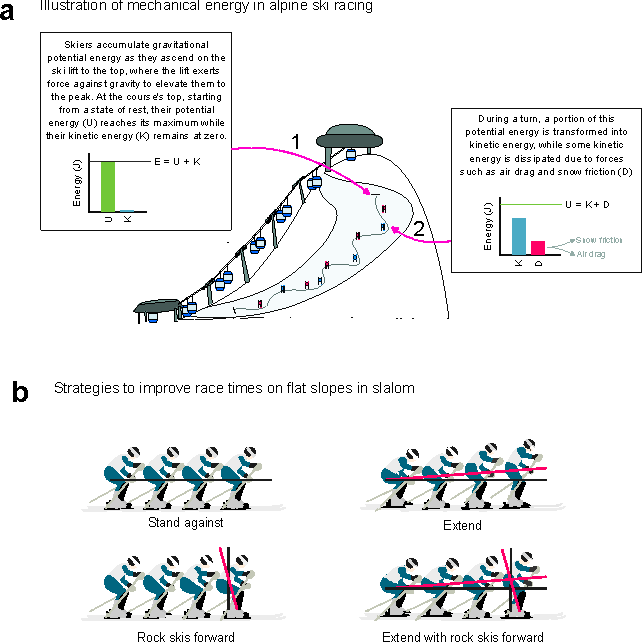
\includegraphics{figure_energymechanics.pdf}
\caption{Kommer}
\label{fig:energy}
\end{figure}

One strategy skiers can exploit to maintain high kinetic energy during a turn and therefore improve their race times on flat sections in slalom is the 'stand against' technique, commonly advocated by many ski coaches. In this technique, skiers maintain a stable stance and actively resist being compressed toward their bindings by centrifugal force during a turn (from the skier's frame of reference). According to Lind and Sander's theoretical model on 'pumping to increase velocity' \cite{lind_physics_2013}, this active force resistance could minimize skiers' kinetic energy loss during a slalom turn by keeping the moment of inertia about the axis of rotation ($I = mr^2$) fixed instead of increasing it, as would occur if the skier collapsed during the turn. In their model, the rotational kinetic energy of a ski turn can be represented by the following equation: 
\[ T = \frac{L^2}{2I} \]
Here, $T$ represents the kinetic energy of rotation, and $L$ represents the angular momentum (that is, angular velocity ($\omega$) multiplied by the moment of inertia about the axis of rotation ($I = mr^2$)). Lind and Sanders considered a rider traveling on a cart on a friction-free rail with a curved turn and no torque to act on the system. In this situation, if the rider were to collapse toward the cart due to the centrifugal force, the moment of inertia would increase by lengthening the radius about the axis of rotation. Consequently, some rotational kinetic energy is lost if the skier fails to resist the centripetal force. Stand against might therefore be an effective strategy to exploit do ski fast on flats in slalom.  

A second and perhaps better strategy skiers can employ to maintain high kinetic energy during a turn is to 'rock skis forward'. By shifting their vertical position forward and backward, skiers regulate the ski’s total pressure distribution against the snow\cite{lemaster_skiers_1999, lemaster_ultimate_2010, howe_new_2001}. This regulation not only helps skiers maintain balance but also affects the ski's turning behavior. For example, when skiers edge their skis, moving the center of mass toward the tip of the ski increases the pressure distribution on the ski's forebody, enabling it to turn more sharply. Conversely, if skiers edge their skis but shift their center of mass backward to the ski's tail, they decrease the pressure at the ski's forebody and consequently make the turn more gradual \cite{lemaster_skiers_1999, lemaster_ultimate_2010}. In ski racing, skiers generally aim to turn more sharply in the beginning and during the turn and should therefore shift their center of mass to distribute the pressure to the ski's forebody to make it engage with the snow. However, after gate passage, skiers generally aim to stop turning and should therefore shift their center of mass backward by rocking the skis forward. By rocking the skis forward after gate passage, skiers could in principle counteract the unnecessary loss of kinetic energy caused by the skis penetrating and digging unnecessarily into the snow in the exit of the turn. In support of this, previous research has found a strong linear relationship between the skier's forward position and energy dissipation \cite{reid_turn_2009}. Additionally, faster skiers have shown to rock their skis more forward and pressure the back part of the ski for considerably longer during a turn compared to slower skiers\cite{reid_kinematic_2010, tjorhom_beskrivelse_2007}. Consequently, rocking skis forward could be an even more effective strategy than the stand against strategy for improving race times on flat terrain in slalom 

The third strategy that can potentially make skiers faster on flat slopes in slalom is to 'extend,' also referred to as 'pumping' to increase velocity \cite{lind_physics_2013}. By moving closer to the axis of rotation of a turn from a laterally inclined position, the skier can boost its kinetic rotational energy under certain situations. According to Lind and Sanders \cite{lind_physics_2013} model, the skier achieves this effect by shortening the radius of the axis about which they rotate, which will reduce the moment of inertia and consequently increase the rotational kinetic energy of the system under the assumption that angular momentum is conserved. In their model, the gain in rotational kinetic energy from this motion is proportional to the amount of work the skier does against the centrifugal force; therefore, a larger extension movement will accomplish a greater increase in rotational kinetic energy. Scientists have previously assumed that the contribution of pumping to increase the velocity through a turn is minimal and an negotiable mechanism to leverage to improve skiers' race times\cite{supej_differential_2008}. Critics are directed that Lind and Sander's model neglects friction and that it only should work with low speeds \cite{supej_differential_2008, supej_how_2010}. Nevertheless, several studies has been observed that skilled alpine skiers gain additional kinetic energy at the exit of the turn—an increase that cannot be accounted for solely by their available potential energy at that moment\cite{reid_kinematic_2010, supej_how_2010, supej_differential_2008}. Moreover, in an experiment we conducted in 2012, elite skiers had better race times on a flat slalom section when they skied the course with the pumping technique than when they skied the section straight down, despite taking a significant longer trajectory in skiing the course. Therefore, "extend" could be a very important strategy.  

The final strategy is to "extend with rock skis forward", which combines "extend" and "rock skis forward". In a simulation study of skiers pumping on a an undulating terrain, this was the the best performing strategy \cite{mote_accelerations_1983}, and it has been suggested that this could be the best strategy to perform in slalom turns in certain situations \cite{reid_kinematic_2010}. We therefore considered this strategy as the theoretical best strategy. 

Selv om det teori og observasjoner av skikjørere i felt som skulle tilsi at 'extend' and 'extend with rock skis forward' skulle være effektive strategier, finnes det ingen eller lite eksperimentelt arbeid for å estimere effektene av disse strategiene på prestasjoner i flate deler av en slalåmløype. Om pumping gjennom strekking er en effektiv strategi for å kjøre fort på flater, er det også interessant å undersøke de kinematiske endringene i en utøveres skikjøring som følge av en intervensjon på pumping. 


\subsection{Why do skilled performers perform better?}
The final stage in the expert performance approach is to understand how. Dette skal jeg diskutere med Romy tenkte jeg. Men svaret på hvorfor utøvere gjør det bedre er relatert til læringsstudiene. Så her skal jeg bygge opp til de to læringsstudien vi har gjort.

\subsection{What is motor skill learning?}
Vi har ofte lite utfordring med å identifisere en god prestasjon når vi ser det. For eksempel kan vi si at en alpinist som kjører rene og raske svinger ned et bratt og isete heng i slalåm for å være skilled. Til tross for dette, klarer ikke forskere å enes om en bestemt definisjon hva det er. Noen forskere har heller forsøkt å snevre inn motor skill learning ved å eksludere hva det ikke er. Ved å gjøre det snakker man ofte om at skilled performance er å utføre en bevegelse snarere enn å kommunisere hva man kan fortelle om ferdigheten. Man skiller også motor skill learning fra adaptasjonsprosesser som ofte blir tilbakestilt med en gang. På et overordnet nivå dreier motorisk læring seg om å successfully achieve goals. Når dette er snakk om motorisk handlinger, snakker vi om motorisk utførelse.

Forskere har på en annen side begynt å lande på hvilke komponenter som inngår i ferdighetslæring. På den ene siden handler det om å velge gode strategier (action selection). For eksempel må en alpinist bestemme seg for om man skal velge en lang linje eller kort linje ned i fart. Når denne strategien er valgt er det viktig at denne handlingen utføres så presist og godt som mulig (action execution). Til slutt er det viktig at disse handlingene utføres så presist som mulig. 

Et kanskje tredje element er å velge gode strategier. Kanskje si noe om de læringmekanismene som støtter dette. 


- Multiple learning mechanism

\subsection{Deliberate practice}
Et viktig aspekt for å utvikle ekspertise er deliberate practice. Deliberate practice kan kjennetegnes ved at å forsøker å hele tiden. Selv om noen. For å få til deliberate practice er det nødvendig med en god oversikt over strategier 



\subsection{Designing practice to make skilled performers learn}


\subsubsection{Contextual interference effect}



%Many studies suggest that training with a high degree of contextual interference can create favorable conditions for learning motor skills (\href{https://www.frontiersin.org/articles/10.3389/fbioe.2022.966041/full\#B28}{Magill and Hall, 1990}; \href{https://www.frontiersin.org/articles/10.3389/fbioe.2022.966041/full\#B23}{Lee and Simon, 2004}; \href{https://www.frontiersin.org/articles/10.3389/fbioe.2022.966041/full\#B29}{Merbah and Meulemans, 2011}). Experiments on the contextual interference effect usually introduce learners to three tasks to be learned (tasks A, B, and C). In the high contextual interference condition (i.e., interleaved practice), the practice order of tasks makes the learner frequently switch between the tasks they acquire (for example, ABC, BAC, or CBA). In contrast, less switching occurs in the low contextual interference condition (i.e., blocked practice) by arranging the tasks in blocks (for example, AAA, CCC, BBB). Previous research has provided evidence that interleaved practice often improves skill preservation over time (i.e., retention) and adaptation of the skill to new situations (i.e., transfer) compared to blocked practice. However, a notable aspect is that blocked practice often results in superior performance during skill acquisition compared to the interleaved group. This paradoxical interaction—called the contextual interference effect—represents a prime example of the distinction between performance and learning in motor learning and has been extensively replicated in a wide variety of scientific laboratory experiments (\href{https://www.frontiersin.org/articles/10.3389/fbioe.2022.966041/full\#B40}{Shea and Morgan, 1979}; \href{https://www.frontiersin.org/articles/10.3389/fbioe.2022.966041/full\#B22}{Lee and Magill, 1983}; \href{https://www.frontiersin.org/articles/10.3389/fbioe.2022.966041/full\#B41}{Simon and Bjork, 2001}; \href{https://www.frontiersin.org/articles/10.3389/fbioe.2022.966041/full\#B47}{Thomas et al., 2021}).

%Despite the existence of ample evidence for the contextual interference effect being present in laboratory environments, it has become clear that the principles deriving from the research do not always generalize to the learning of motor skills in naturalistic settings such as sports (\href{https://www.frontiersin.org/articles/10.3389/fbioe.2022.966041/full\#B52}{Wulf and Shea, 2002}; \href{https://www.frontiersin.org/articles/10.3389/fbioe.2022.966041/full\#B5}{Brady, 2004}; \href{https://www.frontiersin.org/articles/10.3389/fbioe.2022.966041/full\#B2}{Barreiros et al., 2007}). For example, \href{https://www.frontiersin.org/articles/10.3389/fbioe.2022.966041/full\#B2}{Barreiros et al. (2007)} have reported that the proportion of studies showing improved retention due to interleaved practice was considerably smaller for skills performed in a natural environment than for skills performed in a laboratory environment. Furthermore, a meta-analysis showed that the contextual interference effect is typically smaller and more dispersed than in laboratory tasks (\href{https://www.frontiersin.org/articles/10.3389/fbioe.2022.966041/full\#B5}{Brady, 2004}). Therefore, while interleaved practices may improve learning for simple tasks, the evidence for contextual interference for learning more complex tasks in natural environments is not conclusive.

%Over the years, researchers have proposed and examined several different moderators to account for the contradictory results between laboratory and natural environments, including the learner’s age (\href{https://www.frontiersin.org/articles/10.3389/fbioe.2022.966041/full\#B8}{Del Rey et al., 1983}), the amount of practice (\href{https://www.frontiersin.org/articles/10.3389/fbioe.2022.966041/full\#B39}{Shea et al., 1990}), the type of task (\href{https://www.frontiersin.org/articles/10.3389/fbioe.2022.966041/full\#B28}{Magill and Hall, 1990}), the modality-specific requirements of the task (\href{https://www.frontiersin.org/articles/10.3389/fbioe.2022.966041/full\#B38}{Schöllhorn et al., 2022}), and the learner’s skill level relative to the difficulty of the task (\href{https://www.frontiersin.org/articles/10.3389/fbioe.2022.966041/full\#B52}{Wulf and Shea, 2002}; \href{https://www.frontiersin.org/articles/10.3389/fbioe.2022.966041/full\#B16}{Guadagnoli and Lee, 2004}). Concerning the latter of these moderators, the challenge-point framework (\href{https://www.frontiersin.org/articles/10.3389/fbioe.2022.966041/full\#B16}{Guadagnoli and Lee, 2004}) posits that the efficacy of interleaved practice depends on the difficulty of the task as it is objectively defined (that is, nominal task difficulty) but also how challenging the task is relative to the learner’s skill level and practice environment (that is, functional task difficulty). The framework predicts that an interleaved practice may be more beneficial to promoting learning in a context involving learning a task with low nominal difficulty (for example, a simple laboratory task). This expected observation is because interleaved practice increases the functional difficulty of the task to engage the cognitive mechanisms responsible for causing the contextual effect. With more nominally difficult tasks, the task’s characteristic may already be sufficiently challenging to achieve this end so that beginners may benefit from the blocked practice. However, as learners become better at the task, increasing the functional difficulty of the task through interleaved practice may be needed to engage the cognitive mechanisms to promote additive learning. In support of the challenge-point framework, several studies have provided evidence that providing beginners with a gradual and systematic increase in contextual interference when learning complex skills seem to be a better learning approach than the sole use of blocked or interleaved practice (\href{https://www.frontiersin.org/articles/10.3389/fbioe.2022.966041/full\#B32}{Porter and Magill, 2010}; \href{https://www.frontiersin.org/articles/10.3389/fbioe.2022.966041/full\#B36}{Saemi et al., 2012}). These findings suggest that the optimal practice condition changes with the learner’s proficiency and the skill’s complexity.

%The challenge point framework and the supporting evidence that the learner’s skill level interacts with the characteristic of the task in determining the contextual interference effect can build the impression that skilled performers benefit from training with a high degree of contextual interference when improving or refining their skills. Even though some researchers have advocated such an approach (\href{https://www.frontiersin.org/articles/10.3389/fbioe.2022.966041/full\#B7}{Christina and Bjork, 1991}; \href{https://www.frontiersin.org/articles/10.3389/fbioe.2022.966041/full\#B37}{Schmidt, 1991}), few studies have explicitly tested it. One of the few exceptions is a study on skilled baseball players who performed additional batting training to probe the contextual interference effect (\href{https://www.frontiersin.org/articles/10.3389/fbioe.2022.966041/full\#B17}{Hall et al., 1994}). Three groups practiced batting with three types of baseball pitches. The blocked group practiced these pitches in a blocked order (AAA, BBB, CCC), whereas the interleaved group practiced them in a random order (BCA, ABC, BAC). At the end of the training intervention, the interleaved group performed better than the blocked group. This study demonstrated that interleaved practice might also improve learning for skilled performers. It is important to note that \href{https://www.frontiersin.org/articles/10.3389/fbioe.2022.966041/full\#B17}{Hall et al. (1994)} used variations of a single skill (i.e., batting) to probe the contextual interference effect. In a recent study, \href{https://www.frontiersin.org/articles/10.3389/fbioe.2022.966041/full\#B6}{Buszard et al. (2017)} performed a between-skill manipulation to examine the contextual interference effect in youth tennis players. While interleaving the practice schedule did not improve retention for these players compared to the blocked practice schedule on the same task, there was evidence that the interleaved group transferred their skill better to competition (i.e., transfer). Hence, it remains unclear whether training with contextual interference improves learning for skilled performers when improving their skills. This lack of understanding is critical to address in order to provide proper recommendations for instructors in sports and other motor activities, such as surgical operations in medicine and the training of military personnel.

%Testing the contextual interference effect on skilled performers implies specific challenges that must be overcome and effectively solved. The biggest challenge is that skilled performers are usually obsessed with achieving success in their activity and devote significant amounts of their time and resources to improving their performance in this activity. Therefore, recruiting them for a study is often challenging because of their reluctance to modify their training for an experiment, especially if it does not lead to immediate performance gains (\href{https://www.frontiersin.org/articles/10.3389/fbioe.2022.966041/full\#B10}{Farrow and Buszard, 2017}). Even if performers were willing to participate, it would often require a large volume of practice to improve the performance of a skilled practitioner compared to a novice performer (\href{https://www.frontiersin.org/articles/10.3389/fbioe.2022.966041/full\#B17}{Hall et al., 1994}). Hence, even if interleaved practice makes the training more effective, the effect may only become visible after extensive practice, regardless of the skills training method. A final obstacle is that it is often difficult to achieve a robust and sensitive performance goal, especially in alpine ski racing, where external conditions such as snow and wind vary considerably and may influence performance (\href{https://www.frontiersin.org/articles/10.3389/fbioe.2022.966041/full\#B50}{Williams et al., 2017}). Overcoming these challenges requires in-depth knowledge of the skill domain, and real-world practitioner skills are needed to invent innovative approaches to assess skills and deal with issues of validity at the same time (\href{https://www.frontiersin.org/articles/10.3389/fbioe.2022.966041/full\#B10}{Farrow and Buszard, 2017}).

%Considering the need for a better understanding of how the contextual interference effect translates to skilled learners, and how to cope with the described challenges, we have investigated the contextual interference effect on skilled athletes in the complex sport of alpine ski racing in this study. Alpine ski racing is a sport where performance is measured as the time from start to finish, where athletes need to pass through a pre-defined course marked with gates. The sport consists of six main disciplines: slalom (SL), giant-slalom (GS), super-G (SG), downhill (DH), Parallel and Combined, which vary in the number of direction changes,timing and dynamics in turns,terrain and transitions, course length, and jumps (\href{https://www.frontiersin.org/articles/10.3389/fbioe.2022.966041/full\#B15}{Gilgien et al., 2018}). Of these six disciplines, slalom skiing is the most technically demanding due to its frequent changes of direction, high turn forces, and small turn radii (\href{https://www.frontiersin.org/articles/10.3389/fbioe.2022.966041/full\#B35}{Reid, 2010}). Slalom courses generally comprise ∼50 gates, adjacently positioned with a linear distance of 6–13 m. These courses can vary extensively between races depending on the course setter, usually a coach who can determine the type of course within the rules of Fédération International de Ski (FIS). Besides the variability in courses, there is also large variability in terrain characteristics (for example, incline and terrain transitions), snow properties, and weather (for example, visibility). Slalom racers should therefore expect a significant degree of variability in conditions in the performance arena.

%Although the total time differences between skiers in slalom races can be quite small, section differences through a course can be quite significant while typically equalizing to small differences at the finish (\href{https://www.frontiersin.org/articles/10.3389/fbioe.2022.966041/full\#B44}{Supej and Cernigoj, 2006}; \href{https://www.frontiersin.org/articles/10.3389/fbioe.2022.966041/full\#B46}{Supej and Holmberg, 2011}). The sections of slalom courses where significant time differences typically occur between skiers are flat terrain sections (\href{https://www.frontiersin.org/articles/10.3389/fbioe.2022.966041/full\#B44}{Supej and Cernigoj, 2006}). An essential characteristic of flat sections is that the component of gravity that accelerates the skiers downhill is small (\href{https://www.frontiersin.org/articles/10.3389/fbioe.2022.966041/full\#B35}{Reid, 2010}). Therefore, the skier must make the necessary adjustments to their technique to ski fast in this type of terrain (\href{https://www.frontiersin.org/articles/10.3389/fbioe.2022.966041/full\#B45}{Supej et al., 2015}). One technique proposed to help increase speed in flat terrain is to “pump” while turning to increase the turn exit speed (\href{https://www.frontiersin.org/articles/10.3389/fbioe.2022.966041/full\#B30}{Mote and Louie, 1983}; \href{https://www.frontiersin.org/articles/10.3389/fbioe.2022.966041/full\#B25}{Lind and Sanders, 2004}). In this context, pumping refers to the technique of extending the legs and pushing the center of mass towards the axis of rotation at the center of the turn. Through the conservation of angular momentum, pushing the center of mass closer to the axis of rotation can lead to increased tangential velocity (\href{https://www.frontiersin.org/articles/10.3389/fbioe.2022.966041/full\#B25}{Lind and Sanders, 2004}). Therefore, the extent and quality with which skiers can exploit this technique can be a primary explanation for the time differences in flat sections.

%Because the technique that leads to good performance differs depending on the terrain incline, researchers have recommended dividing training into sessions with uniform terrain inclines to achieve more element-focused training (\href{https://www.frontiersin.org/articles/10.3389/fbioe.2022.966041/full\#B45}{Supej et al., 2015}). Once training in a section of uniform terrain incline, coaches need to determine the slalom gates’ location down the hill. The location of the gates determines two characteristics of the course: the linear distance between successive gates determines the room skiers have for turning between gates, and the offset determines how “turny” the course is. Changes in these two course dimensions can cause significant changes in the required technique, and the tactics skiers must use to ski the course. For example, changes in gate offset have been shown to reduce speed and turn radius but increase turn forces, impulse (a measure of physical load), and inward lean for giant slalom and super-G (\href{https://www.frontiersin.org/articles/10.3389/fbioe.2022.966041/full\#B43}{Spörri et al., 2012}; \href{https://www.frontiersin.org/articles/10.3389/fbioe.2022.966041/full\#B13}{Gilgien et al., 2020}, \href{https://www.frontiersin.org/articles/10.3389/fbioe.2022.966041/full\#B12}{Gilgien et al., 2021}). In contrast, shortening the linear distance between gates causes a reduction in turn time and speed but has a limited effect on forces and turn radii compared to changes in the offset (\href{https://www.frontiersin.org/articles/10.3389/fbioe.2022.966041/full\#B35}{Reid, 2010}; \href{https://www.frontiersin.org/articles/10.3389/fbioe.2022.966041/full\#B13}{Gilgien et al., 2020}, \href{https://www.frontiersin.org/articles/10.3389/fbioe.2022.966041/full\#B12}{2021}). Because course setting has a significant impact on skiers’ technique and is the training variable that coaches can influence the most, there is a general conception that this is one of the most critical variables affecting learning.

%Because skiers never know what courses and conditions to expect in a race, they must master an extensive range of conditions. Therefore, undertaking training to perfect performance in a single course setting may not be effective. Instead, researchers have argued that a better approach is to use interleaved practice in these types of open sports (\href{https://www.frontiersin.org/articles/10.3389/fbioe.2022.966041/full\#B10}{Farrow and Buszard, 2017}). However, few studies have tested this recommendation due to the described challenges of conducting studies on complex learning tasks with skilled performers. Therefore, we established this study to test the contextual interference effect with skilled alpine ski racers in a realistic real-world ski racing environment. An important goal was to do the study with a large number of participants to estimate the contextual interference effect robustly. To achieve this goal, we designed a study that targeted a particular skill element of skiing performance that was relevant for the skiers to improve. Targeting this specific element instead of providing holistic training, we were also able to improve the skiers’ performance by a significant degree, because training this skill was novel for the participants.

%In this study, we expected contextual interference to apply to the training of alpine ski racers. Our rationale for expecting an extension of the effect to this context emerged from previous studies that reported improved retention of continuous skills (cyclic bimanual coordination task) resulting from interleaved compared to blocked practice (\href{https://www.frontiersin.org/articles/10.3389/fbioe.2022.966041/full\#B48}{Tsutsui et al., 1998}; \href{https://www.frontiersin.org/articles/10.3389/fbioe.2022.966041/full\#B31}{Pauwels et al., 2014}). Moreover, in a snow environment, \href{https://www.frontiersin.org/articles/10.3389/fbioe.2022.966041/full\#B42}{Smith (2002)} reported that novices learned snowboarding turns better after practicing four different turns (left/right and heel/toe) in an interleaved compared to a blocked order. This finding suggests that contextual interference may be relevant for learning skills in alpine ski racing. If skiers vary their turns in an interleaved manner, as is accomplished by frequently switching between courses, we could expect to observe contextual interference in alpine skiing. In the snowboarding study, however, the participants were novices, and it is unclear how this extrapolates to skilled performers. Based on the previous research that has provided evidence for the contextual interference for experienced performers (\href{https://www.frontiersin.org/articles/10.3389/fbioe.2022.966041/full\#B17}{Hall et al., 1994}), we hypothesized that interleaved practice would suppress performance during acquisition but improve performance at retention.

 



%What can coaches do to train deliberate practice?






%I den siste fasen forsøker man å finne ut hvordan eksperter tilegner seg ferdighetene for å kjøre for på flater. 


%Deliberate practice and strategies

%Adaptive and skilful

%I





%et viktig innsikt er at. et viktig innsikt ermed hvordan de presterer bedre. er de


%- Tilrettelegging og veiledning


%Organisation, Instruction and feedback


Contextual interference


Reinforcement learning





\subsection{Aims}




\section{Method}

\subsection{Sample and approach}


\section{Results}


\subsection{How do skilled performers perform better on flat section in slalom?}


\subsubsection{Which strategies are best to perform well on flats?}
We began by studying which technical strategies enable skilled alpine skiers to descend a flat slalom course as quickly as possible. The strategies we examined in study 3 were "stand against," "rock skis forward," "extend," and "extend with rock skis forward." We began testing after a familiarizing session where we introduced skiers to the strategies and allowed them to practice until they understood and mastered the techniques. Once understood, the skiers performed a total of eight trials (two on each strategy) that were randomly assigned to each skier under the condition that the first and last four trials included all four strategies. Therefore, we could use the data to estimate which technical strategies enable skilled alpine skiers to descend a flat slalom course as quickly as possible.

We employed a Bayesian modeling approach (model 1) to estimate the differences between the strategies. The analysis revealed that skiers on average achieved their best descent times using the 'extend with rock skis forward' strategy (16.66, 95\% credible interval (CI) = 16.54, 16.77). The second best strategy for skiers was to step down to solely "extend," which was only 0.02 sec. (95\% CI = -0.02, 0.06) slower than the "extend with rock skis forward" strategy. However, when skiers switched from the "extend" strategy to the "rock ski forward" strategy, the expected time loss was 0.21 sec. (95\% CI = 0.16, 0.25). Finally, if the skiers switched from the "rock skis forward" strategy to the "stand against" strategy, the expected time loss was 0.2 sec. (95\% CI = 0.15, 0.25). Therefore, the strategies the skiers used made a great difference in race time.

The results show that just skiing cleanly and resisting centripetal forces during a turn does not suffice to achieve fast race times on flat terrain in slaloms. Instead, the active movements of the skiers were crucial for achieving good race times on flats. "Rock skis forward" resulted in significant improvements in race times compared to 'stand against'. This finding aligns well with prior findings in slalom skiing, showing a strong correlation between fore and aft movements and energy dissipation, such that more fore movements are associated with greater energy dissipation \cite{reid_turn_2009, reid_kinematic_2010}. Furthermore, studies have shown that faster skiers have a greater range of fore/aft motion and spend a larger portion of the turn skiing with their weight shifted back after gate passage than slower skiers \cite{tjorhom_beskrivelse_2007, reid_kinematic_2010}. Our results extend these findings and provide experimental evidence that "rock skis forward" can be an effective strategy for improving race times on flat terrain in slalom.

The 'rock skis forward' strategy resulted in much slower times than did the 'extend' strategy, however. Predictions from the Lind and Sanders model \cite{lind_physics_2013} indicate that extending the center of mass closer to the axis of rotation during a turn from a laterally inclined position should significantly improve the race time. Without motion capture data, we cannot assess the extent to which skiers extended and the resulting increase in kinetic energy. Nonetheless, the results suggest that skiers' extension movements play a crucial role in slalom performance, contrary to previous claims \cite{supej_differential_2008}.

Finally, we found that "extend with rock skis forward" on average was the best strategy. This finding aligns with previous simulations suggesting that this strategy is most effective when skiers pump over rollers \cite{mote_accelerations_1983} and that it can be transferred to skiers executing a turn \cite{reid_kinematic_2010}. However, it is important to emphasize that "extend with rock skis forward" only was marginally better than the "stretching" strategy alone. One reason for the limited improvement achieved by adding "rock skis forward" to the "extend" strategy might be that rocking the skis forward during the turn compromised how much the skier could extend toward the turn's axis of rotation. For instance, extensive extension could be challenging if the skier's center of mass was located at the tail of the skis. This issue should be further investigated in future analyses.

One limitation of these timing analyses is that we do not have precise knowledge of how much the skiers moved when executing the strategies or how these strategies affected the mechanical energy during a turn. Therefore, we cannot comment on the skiers' actual execution or the energy mechanics behind each strategy. Future studies should incorporate motion capture to address this gap in understanding.



\begin{figure}[H]
\centering
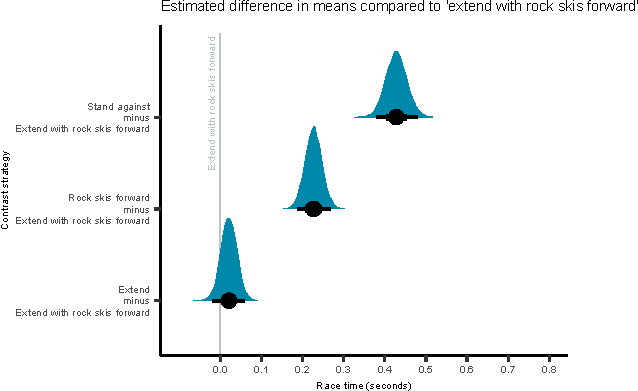
\includegraphics{figure_results_Q1_strategies.pdf}
\caption{Estimated differences in means compared to 'extend with rock skis forward'. The circle represents the point estimates whereas the shaded distribution represents the posterior distribution fitted from the model}
\label{fig:q1_strategieseffect}
\end{figure}

\subsection{Why do they perform better?}
Her tenkte jeg å besvare spørsmålene som har med læring å gjøre

\subsubsection{Contextual interference}

\subsubsection{Reinforcement learning}







\section{General discussion}


\printbibliography

\end{document}
